\chapter{Modeling user-to-user influence on user behavior}
%\chapter{Modeling social influence on user behavior}
\label{chap:social}
In this chapter, we model the influence of the user's explicit social connections and implicit similarity connections on their behavior. Recommender systems are a perfect example of an online platform where user preferences exhibit strong user homophily with their friends. In this work, we exploit homophily in the user and item space. Besides, user's history itself influences their preferences.
We propose separate modules to capture these different factors and later fuse them to predict future items accurately for platform users. Our model outperforms previous approaches modeling a subset of these factors \cite{social}.

\section{Overview}

Recommender systems are ubiquitous and model user preferences on commercial and social websites as well as in apps. These systems predict with reasonable accuracy, products that we may be interested in, people which we may know, or songs and movies that we may appreciate. This success builds upon a long history of research. However, to this day, a large active community continues to improve recommender systems as many questions remain open, e.g., How to effectively model and merge multiple factors influencing user preferences like (1) temporal context, (2) social influence, and (3) similarity between items? We explore this question in detail in this chapter.

Classic collaborative filtering is one of the most successful approaches to model user preferences. It learns a low dimensional and often linear latent factor model for both users and items via matrix factorization of the user-item interaction matrix~\cite{Rendle}. With deep learning taking a more prominent role, more complex models have been applied to learn increasingly non-linear relationships~\cite{NeuMF, CDAE}.
However, those classical methods ignore all three of the factors above.
Hence, many techniques have been developed, which augment classical recommender systems with one of those factors.

First, considering temporal context removes the assumption of a static interaction matrix, which generally doesn't hold as user preferences evolve with time. Thus, history from a distant past is not necessarily relevant to current preferences.
To this end, Markov chains~\cite{Rendle2} and recently, Convolution Neural Network (CNN)~\cite{SAS:2018} and Recurrent Neural Network (RNN)~\cite{GRU4Rec} based methods have been proposed to model this temporal dependence in recommender systems.
Those methods remove the static interaction matrix of classical collaborative filtering and learn a user's and an item's hidden representation based on their recent interactions.

Second, considering social influence removes the restriction that users operate in isolation. This idea is popularized by the social influence theory~\cite{Tang:2009}, which argues that a user's preference is influenced by their friends' behavior, leading to user homophily (similar user preferences). It is noteworthy that these influences are inherently dynamic as friends' preferences are evolving too (socio-temporal influence), a fact mostly ignored by current systems.
For instance, recent works model static social effect~\cite{SBPR, Collaborative, SERec, fan2019}. These methods look at the entire history of the user's friends instead of emphasizing the most recent actions. Moreover, these approaches assume uniform importance of all friends. While this is not suitable in general, it is an important first step to understand social influence for  recommendation.

Third, exploiting similarities between items (based on co-occurrence or similar features)  alleviates the data sparsity issue %for long-tail items
(many items with few ratings). Similar items hold similar attractiveness to users, leading to item homophily. Deep net based recommender models are prone to skew prediction results towards popular items with ample feedback in the training data (overfit to popular items)~\cite{ Longtail:2018}. This is counterproductive to user experience as it leads to similar recommendations across users. Also, compared to highly frequented items, long-tail items (items with fewer ratings) result in higher profit margins for the platforms~\cite{Yin:2012}. Item-Item collaborative filtering based methods~\cite{itemCF} integrate these similarities but ignore the user's history; thus providing generic recommendations.

\begin{figure}[tbh]
  \centering
  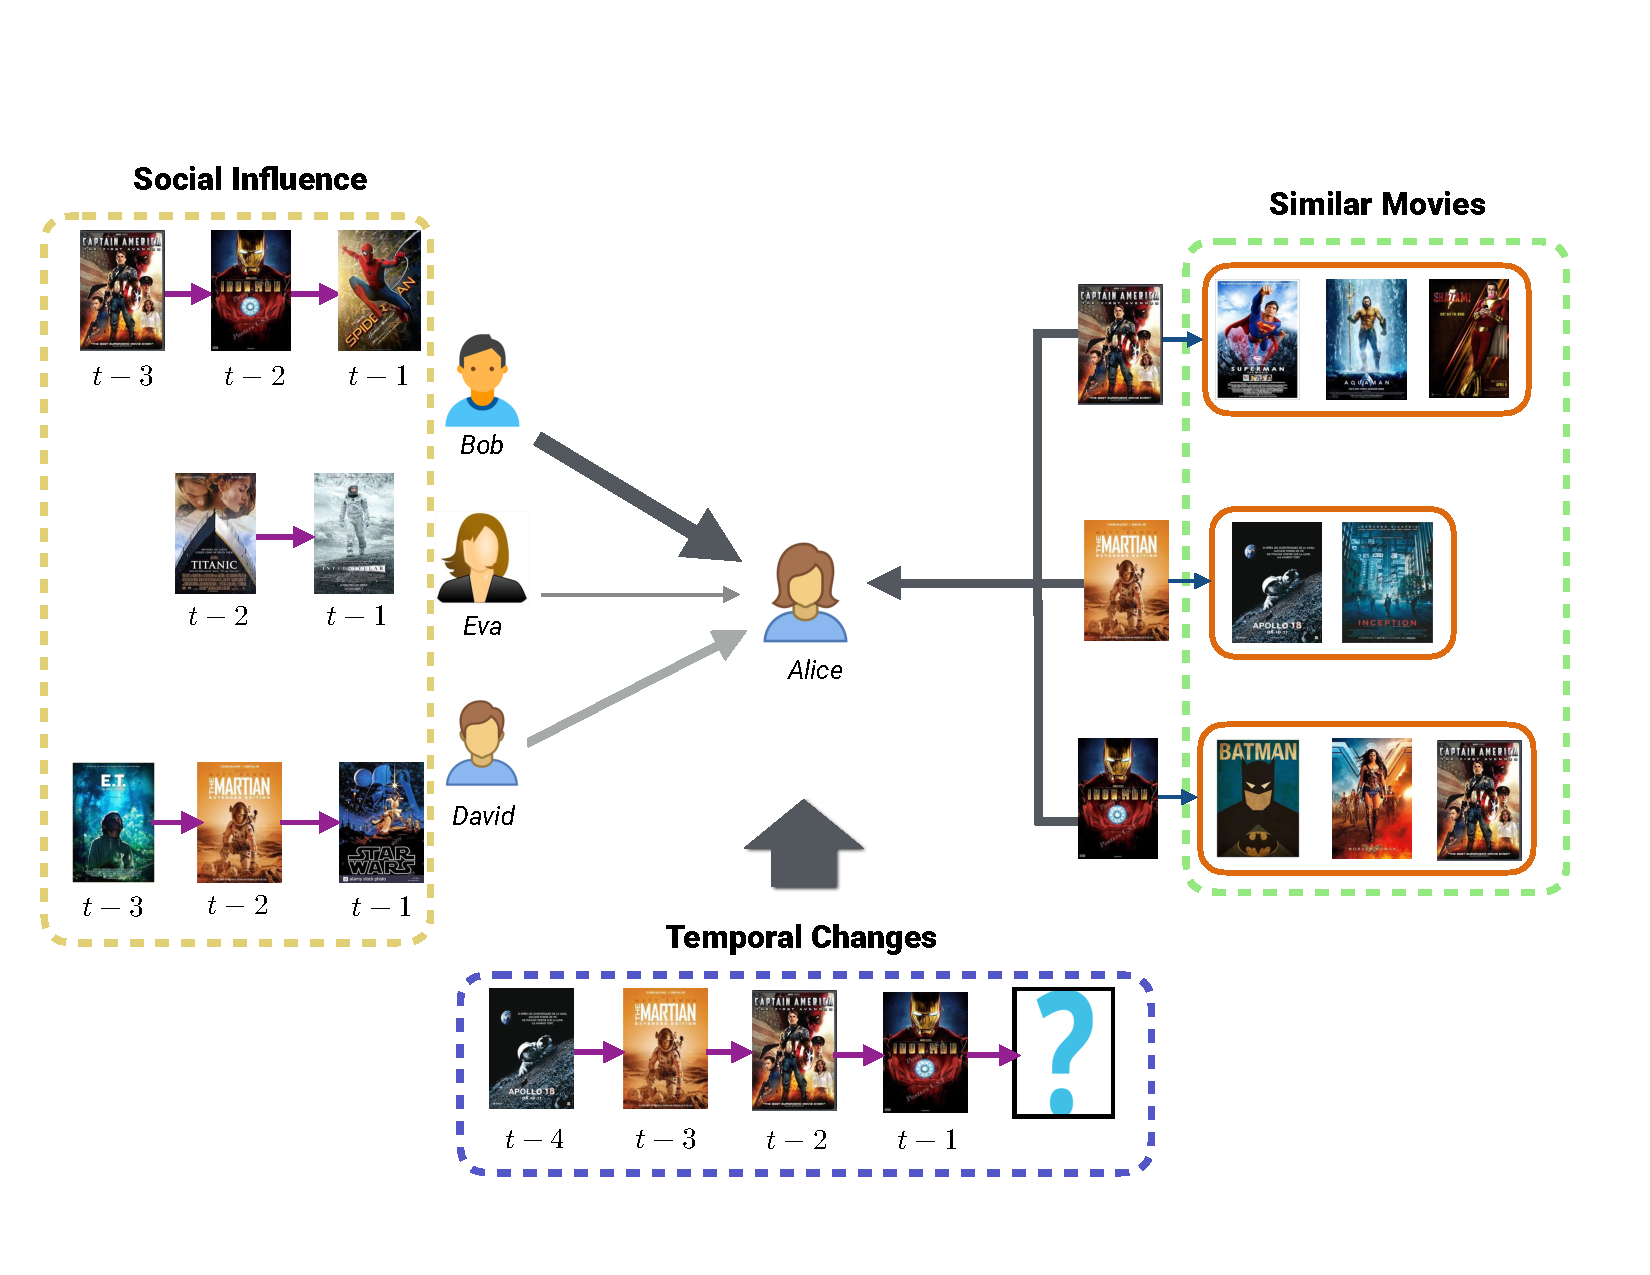
\includegraphics[width=\linewidth]{figures/Idea}
  \caption{Illustrative diagram of factors affecting Alice's decision on which movie to watch next in an online social movie viewing platform. Her current interests are towards superhero movies (temporal); she could either decide to watch recent superhero movies seen by her friends (social) or other superhero movies not watched by her friends (similar items).}
  \label{fig:Idea}
\end{figure}

To make these three points concrete, let us consider the example shown in Figure~\ref{fig:Idea}. Alice is using an online social movie viewing platform. She is currently hooked onto superhero movies (temporal). While deciding which movie to watch next, she will be influenced by recent superhero movies watched by her friends on the platform (socio-temporal influence). She could also decide to watch other superhero movies in the platform not seen by her social circle yet (item-to-item similarity).

As illustrated earlier, a user's behavior is affected by at least
the aforementioned three factors (others could include time-of-day, mood, etc.). However, the relative importance of these factors still remains unclear. It is indeed challenging to model these factors effectively and efficiently in a unified model as these cues mutually influence each other.
This is emphasized by the fact that existing work often studies only a subset of those three cues.

To address this concern, we develop a `Fusion Recommender' (FuseRec) model to jointly and efficiently capture all the factors in a unified model. It takes into account a user's temporal changes along with homophily in the user and item space. It treats each of the signals equally and combines them in an interpretable manner.

More specifically, we use three different modules to model each factor: (1) a user-temporal, (2) a user-social, and (3) an item-similarity module.
To model the temporal behavior of a user's item viewing history, we use widely adopted recurrent neural nets. These networks are shown to capture complex and non-linear relationships of time-varying sequences. To capture the effect of a user's friends' recent history, we develop a novel attention based social aggregation model. Different from existing works, it aggregates a user's friends' recent item history in a weighted manner. We learn attention weights separately for each pair of a user and her friend.
For item-item similarity aggregation, we construct a `social graph of items' based on similarity in item features and co-occurrence in the dataset. We develop a novel attention based aggregation model for the item similarity graph too.
In contrast to existing work, we learn an attention weight for each similar item and later aggregate information of neighboring items in a weighted manner.

To provide an understanding of the importance of the three factors, we choose to linearly combine them via learned weights. The magnitude of the learned weights permits a glimpse at the importance of the individual modules.


We evaluate our model on three representative benchmark datasets: Ciao, CiaoDVD, and Epinions. We compare to an array of collaborative filtering, temporal, and social methods and achieve a significant improvement of more than 14\% for AUC on the Ciao and the Epinions dataset and around 2\% for the CiaoDVD dataset. In addition, we provide a study on the importance of the three factors. Across all datasets, we find the temporal module to be the most significant factor for modeling user preferences.

In summary, our main contributions are as follows:
\begin{itemize}
    \item We propose `FuseRec,' a Fusion Recommender model which combines temporal, social, and item similarity aspects in an interpretable manner.
    \item  We propose a novel attention based aggregation model to capture homophily in the user and item space.
    \item We evaluate our method on three benchmark datasets and compare to a variety of recent temporal, social, and socio-temporal models.
    \item We provide a detailed study regarding the importance of different factors used in our model.
\end{itemize}
